\documentclass[11pt,a4paper]{article}
\usepackage[margin=2.2cm]{geometry}
\usepackage{amsmath}
\usepackage{lmodern}
\usepackage{tikz}
\setcounter{secnumdepth}{0}
\pagestyle{empty}

\begin{document}

\begin{center}
{\fontsize{16}{19.2}\selectfont\bfseries Euler--Lagrange derivation (2-arm pendulum)}
\end{center}

\[ L = T - V \]

\section{Setup}

Pivot at the origin. Generalized coordinates: the absolute angles $\theta_1, \theta_2$.
Screen convention: $(0,0)$ is the top-left corner, so $y$ increases downward.

\begin{center}
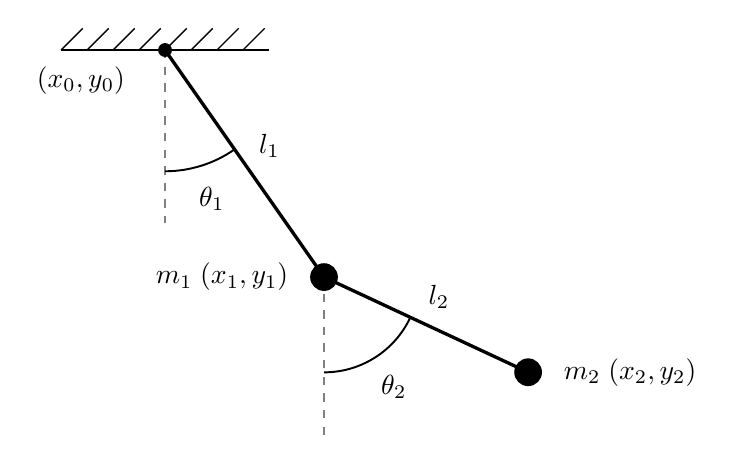
\begin{tikzpicture}[scale=1.1]
  \pgfmathsetmacro{\thA}{35}
  \pgfmathsetmacro{\thB}{65}
  \pgfmathsetmacro{\lA}{3.2}
  \pgfmathsetmacro{\lB}{2.6}
  \pgfmathsetmacro{\pax}{\lA*sin(\thA)}
  \pgfmathsetmacro{\pay}{-\lA*cos(\thA)}
  \pgfmathsetmacro{\pbx}{\pax + \lB*sin(\thB)}
  \pgfmathsetmacro{\pby}{\pay - \lB*cos(\thB)}

  % ceiling with hatching
  \draw (-1.2, 0) -- (1.2, 0);
  \foreach \i in {0,...,7} {
    \draw[line width=0.5pt] ({-1.2 + \i*0.3}, 0) -- ({-1.2 + \i*0.3 + 0.25}, 0.25);
  }

  % dashed vertical reference lines
  \draw[dashed, gray] (0, 0) -- (0, -2.0);
  \draw[dashed, gray] (\pax, \pay) -- (\pax, \pay - 1.9);

  % angle arcs (measured from the downward vertical)
  \draw[line width=0.7pt] (0, -1.4) arc[start angle=-90, end angle={-90 + \thA}, radius=1.4];
  \node at ({1.8*sin(\thA/2)}, {-1.8*cos(\thA/2)}) {$\theta_1$};
  \draw[line width=0.7pt] (\pax, \pay - 1.1) arc[start angle=-90, end angle={-90 + \thB}, radius=1.1];
  \node at ({\pax + 1.5*sin(\thB/2)}, {\pay - 1.5*cos(\thB/2)}) {$\theta_2$};

  % arms
  \draw[line width=1.2pt] (0, 0) -- (\pax, \pay);
  \draw[line width=1.2pt] (\pax, \pay) -- (\pbx, \pby);

  % arm length labels (offset perpendicular to each arm)
  \node at ({\pax/2 + 0.35*cos(\thA)}, {\pay/2 + 0.35*sin(\thA)}) {$l_1$};
  \node at ({(\pax + \pbx)/2 + 0.35*cos(\thB)}, {(\pay + \pby)/2 + 0.35*sin(\thB)}) {$l_2$};

  % pivot and masses
  \fill (0, 0) circle[radius=0.08];
  \node[anchor=east] at (-0.35, -0.35) {$(x_0, y_0)$};
  \fill (\pax, \pay) circle[radius=0.16];
  \node[anchor=east] at (\pax - 0.3, \pay) {$m_1 \; (x_1, y_1)$};
  \fill (\pbx, \pby) circle[radius=0.16];
  \node[anchor=west] at (\pbx + 0.3, \pby) {$m_2 \; (x_2, y_2)$};
\end{tikzpicture}
\end{center}

\section{Positions}

\[ x_1 = x_0 + l_1 \sin\theta_1 \qquad y_1 = y_0 + l_1 \cos\theta_1 \]

\[ x_2 = x_1 + l_2 \sin\theta_2 \qquad y_2 = y_1 + l_2 \cos\theta_2 \]

\section{Velocities}

\[ \dot{x}_1 = l_1 \cos\theta_1 \, \dot{\theta}_1 \qquad \dot{y}_1 = -l_1 \sin\theta_1 \, \dot{\theta}_1 \]

\[ v_1 = \sqrt{\dot{x}_1^2 + \dot{y}_2^2} \qquad v_1^2 = \dot{x}_1^2 + \dot{y}_1^2 \]

\[ \dot{x}_2 = \dot{x}_1 + l_2 \cos\theta_2 \, \dot{\theta}_2 \qquad \dot{y}_2 = \dot{y}_1 - l_2 \sin\theta_2 \, \dot{\theta}_2 \]

\[ v_2 = \sqrt{\dot{x}_2^2 + \dot{y}_2^2} \qquad v_2^2 = \dot{x}_2^2 + \dot{y}_2^2 \]

\section{Kinetic energy}

\[ T = \frac{1}{2} m v^2 \qquad \Longrightarrow \qquad T = \frac{1}{2} m_1 v_1^2 + \frac{1}{2} m_2 v_2^2 \]

\section{Potential energy}

\[ V = m g h, \qquad h_1 = -y_1, \quad h_2 = -y_2 \]

\[ V = g (m_1 h_1 + m_2 h_2) \]

\[ V = -g (m_1 y_1 + m_2 y_2) \]

\section{Lagrangian}

\[ L = T - V \]

\[ L = \frac{1}{2} (m_1 v_1^2 + m_2 v_2^2) - g (m_1 h_1 + m_2 h_2) \]

\[ L = \frac{1}{2} \left( m_1 (\dot{x}_1^2 + \dot{y}_1^2) + m_2 (\dot{x}_2^2 + \dot{y}_2^2) \right) - g (m_1 - y_1 + m_2 - y_2) \]

Substituting the velocities:

\begin{align*}
L &= \frac{1}{2} m_1 \left( (\cos\theta_1 \, l_1 \dot{\theta}_1)^2 + (-\sin\theta_1 \, l_1 \dot{\theta}_1)^2 \right) \\
  &\quad + \frac{1}{2} m_2 \left( (\dot{x}_1 + \cos\theta_2 \, l_2 \dot{\theta}_2)^2 + (\dot{y}_1 - \sin\theta_2 \, l_2 \dot{\theta}_2)^2 \right) \\
  &\quad + g \left( m_1 y_1 + m_2 y_2 \right)
\end{align*}

\begin{align*}
L &= \frac{1}{2} m_1 \left( (\cos\theta_1 \, l_1 \dot{\theta}_1)^2 + (-\sin\theta_1 \, l_1 \dot{\theta}_1)^2 \right) \\
  &\quad + \frac{1}{2} m_2 \left( (\cos\theta_1 \, l_1 \dot{\theta}_1 + \cos\theta_2 \, l_2 \dot{\theta}_2)^2 + (-\sin\theta_1 \, l_1 \dot{\theta}_1 - \sin\theta_2 \, l_2 \dot{\theta}_2)^2 \right) \\
  &\quad + g \left( m_1 (y_0 + \cos\theta_1 \, l_1) + m_2 (y_1 + \cos\theta_2 \, l_2) \right)
\end{align*}

Expanding the squares:

\begin{align*}
L &= \frac{1}{2} m_1 \left( \cos^2\theta_1 \, l_1^2 \dot{\theta}_1^2 + \sin^2\theta_1 \, l_1^2 \dot{\theta}_1^2 \right) \\
  &\quad + \frac{1}{2} m_2 \big( \cos^2\theta_1 \, l_1^2 \dot{\theta}_1^2 + 2 \cos\theta_1 \, l_1 \dot{\theta}_1 \cos\theta_2 \, l_2 \dot{\theta}_2 + \cos^2\theta_2 \, l_2^2 \dot{\theta}_2^2 \\
  &\quad\quad\quad + \sin^2\theta_1 \, l_1^2 \dot{\theta}_1^2 + 2 \sin\theta_1 \, l_1 \dot{\theta}_1 \sin\theta_2 \, l_2 \dot{\theta}_2 + \sin^2\theta_2 \, l_2^2 \dot{\theta}_2^2 \big) \\
  &\quad + g \left( m_1 (y_0 + \cos\theta_1 \, l_1) + m_2 (y_1 + \cos\theta_2 \, l_2) \right)
\end{align*}

Grouping:

\begin{align*}
L &= \frac{1}{2} m_1 l_1^2 \dot{\theta}_1^2 (\cos^2\theta_1 + \sin^2\theta_1) \\
  &\quad + \frac{1}{2} m_2 \big( l_1^2 \dot{\theta}_1^2 (\cos^2\theta_1 + \sin^2\theta_1) + l_2^2 \dot{\theta}_2^2 (\cos^2\theta_2 + \sin^2\theta_2) \\
  &\quad\quad\quad + 2 l_1 \dot{\theta}_1 l_2 \dot{\theta}_2 (\cos\theta_1 \cos\theta_2 + \sin\theta_1 \sin\theta_2) \big) \\
  &\quad + g \left( m_1 (y_0 + \cos\theta_1 \, l_1) + m_2 (y_1 + \cos\theta_2 \, l_2) \right)
\end{align*}

Using $\cos^2 + \sin^2 = 1$ and $\cos\theta_1 \cos\theta_2 + \sin\theta_1 \sin\theta_2 = \cos(\theta_1 - \theta_2)$:

\begin{align*}
L &= \frac{1}{2} m_1 l_1^2 \dot{\theta}_1^2 \\
  &\quad + \frac{1}{2} m_2 \left( l_1^2 \dot{\theta}_1^2 + l_2^2 \dot{\theta}_2^2 + 2 l_1 l_2 \dot{\theta}_1 \dot{\theta}_2 \cos(\theta_1 - \theta_2) \right) \\
  &\quad + g \left( m_1 (y_0 + l_1 \cos\theta_1) + m_2 (y_0 + l_1 \cos\theta_1 + l_2 \cos\theta_2) \right)
\end{align*}

\section{Euler--Lagrange}

\[ \frac{d}{dt} \left( \frac{\partial L}{\partial \dot{q}} \right) - \frac{\partial L}{\partial q} = 0 \]

\subsection{For $\theta_1$}

\[ \frac{d}{dt} \left( \frac{\partial L}{\partial \dot{\theta}_1} \right) - \frac{\partial L}{\partial \theta_1} = 0 \]

First $\partial L / \partial \theta_1$:

\begin{align*}
\frac{\partial L}{\partial \theta_1} = \frac{\partial}{\partial \theta_1} \Big[
  &\frac{1}{2} m_1 l_1^2 \dot{\theta}_1^2 \\
  &+ \frac{1}{2} m_2 \left( l_1^2 \dot{\theta}_1^2 + l_2^2 \dot{\theta}_2^2 + 2 l_1 l_2 \dot{\theta}_1 \dot{\theta}_2 \cos(\theta_1 - \theta_2) \right) \\
  &+ g \left( m_1 (y_0 + l_1 \cos\theta_1) + m_2 (y_0 + l_1 \cos\theta_1 + l_2 \cos\theta_2) \right) \Big]
\end{align*}

\[ \frac{\partial L}{\partial \theta_1} = \frac{1}{2} m_2 \left( 2 l_1 l_2 \dot{\theta}_1 \dot{\theta}_2 (-\sin(\theta_1 - \theta_2)) \right) + g \left( m_1 l_1 (-\sin\theta_1) + m_2 l_1 (-\sin\theta_1) \right) \]

\[ \frac{\partial L}{\partial \theta_1} = -m_2 l_1 l_2 \dot{\theta}_1 \dot{\theta}_2 \sin(\theta_1 - \theta_2) - g l_1 (m_1 + m_2) \sin\theta_1 \]

Then $\partial L / \partial \dot{\theta}_1$:

\[ \frac{\partial L}{\partial \dot{\theta}_1} = m_1 l_1^2 \dot{\theta}_1 + \frac{1}{2} m_2 \left( 2 l_1^2 \dot{\theta}_1 + 2 l_1 l_2 \dot{\theta}_2 \cos(\theta_1 - \theta_2) \right) \]

\[ \frac{\partial L}{\partial \dot{\theta}_1} = m_1 l_1^2 \dot{\theta}_1 + m_2 l_1 \left( l_1 \dot{\theta}_1 + l_2 \dot{\theta}_2 \cos(\theta_1 - \theta_2) \right) \]

\begin{align*}
\frac{d}{dt} \left( \frac{\partial L}{\partial \dot{\theta}_1} \right)
  &= m_1 l_1^2 \ddot{\theta}_1 \\
  &\quad + m_2 l_1 \left( l_1 \ddot{\theta}_1 + l_2 \left( \ddot{\theta}_2 \cos(\theta_1 - \theta_2) + \dot{\theta}_2 (-\sin(\theta_1 - \theta_2) (\dot{\theta}_1 - \dot{\theta}_2)) \right) \right)
\end{align*}

Combining and simplifying:

\begin{align*}
& m_1 l_1^2 \ddot{\theta}_1 + m_2 l_1 \left( l_1 \ddot{\theta}_1 + l_2 \left( \ddot{\theta}_2 \cos(\theta_1 - \theta_2) + \dot{\theta}_2 (-\sin(\theta_1 - \theta_2) (\dot{\theta}_1 - \dot{\theta}_2)) \right) \right) \\
&\quad - \left( m_2 l_1 \dot{\theta}_1 l_2 \dot{\theta}_2 (-\sin(\theta_1 - \theta_2)) + g l_1 (-\sin\theta_1) (m_1 + m_2) \right) = 0
\end{align*}

\begin{align*}
& m_1 l_1^2 \ddot{\theta}_1 + m_2 l_1^2 \ddot{\theta}_1 + m_2 l_1 l_2 \left( \ddot{\theta}_2 \cos(\theta_1 - \theta_2) + \dot{\theta}_2 (-\sin(\theta_1 - \theta_2) (\dot{\theta}_1 - \dot{\theta}_2)) \right) \\
&\quad - m_2 l_1 \dot{\theta}_1 l_2 \dot{\theta}_2 (-\sin(\theta_1 - \theta_2)) - g l_1 (-\sin\theta_1) (m_1 + m_2) = 0
\end{align*}

\begin{align*}
& (m_1 + m_2) l_1^2 \ddot{\theta}_1 + m_2 l_1 l_2 \ddot{\theta}_2 \cos(\theta_1 - \theta_2) \\
&\quad + m_2 l_1 l_2 \dot{\theta}_2 (-\sin(\theta_1 - \theta_2)) (\dot{\theta}_1 - \dot{\theta}_2) \\
&\quad - m_2 l_1 l_2 \dot{\theta}_2 \dot{\theta}_1 (-\sin(\theta_1 - \theta_2)) \\
&\quad - g l_1 (-\sin\theta_1) (m_1 + m_2) = 0
\end{align*}

\begin{align*}
& (m_1 + m_2) l_1^2 \ddot{\theta}_1 + m_2 l_1 l_2 \ddot{\theta}_2 \cos(\theta_1 - \theta_2) \\
&\quad + m_2 l_1 l_2 \dot{\theta}_2 (-\sin(\theta_1 - \theta_2)) \left( (\dot{\theta}_1 - \dot{\theta}_2) - \dot{\theta}_1 \right) \\
&\quad - g l_1 (-\sin\theta_1) (m_1 + m_2) = 0
\end{align*}

\textbf{Euler--Lagrange equation for $\theta_1$:}

\begin{align*}
(m_1 + m_2) l_1^2 \ddot{\theta}_1 &+ m_2 l_1 l_2 \ddot{\theta}_2 \cos(\theta_1 - \theta_2) \\
  &= -g l_1 (m_1 + m_2) \sin\theta_1 - m_2 l_1 l_2 \dot{\theta}_2^2 \sin(\theta_1 - \theta_2)
\end{align*}

\subsection{For $\theta_2$}

\[ \frac{d}{dt} \left( \frac{\partial L}{\partial \dot{\theta}_2} \right) - \frac{\partial L}{\partial \theta_2} = 0 \]

First $\partial L / \partial \theta_2$:

\begin{align*}
\frac{\partial L}{\partial \theta_2} = \frac{\partial}{\partial \theta_2} \Big[
  &\frac{1}{2} m_1 l_1^2 \dot{\theta}_1^2 \\
  &+ \frac{1}{2} m_2 \left( l_1^2 \dot{\theta}_1^2 + l_2^2 \dot{\theta}_2^2 + 2 l_1 l_2 \dot{\theta}_1 \dot{\theta}_2 \cos(\theta_1 - \theta_2) \right) \\
  &+ g \left( m_1 (y_0 + l_1 \cos\theta_1) + m_2 (y_0 + l_1 \cos\theta_1 + l_2 \cos\theta_2) \right) \Big]
\end{align*}

\[ \frac{\partial L}{\partial \theta_2} = \frac{1}{2} m_2 \left( 2 l_1 l_2 \dot{\theta}_1 \dot{\theta}_2 (-\sin(\theta_1 - \theta_2) \cdot (-1)) \right) + g \left( m_2 l_2 (-\sin\theta_2) \right) \]

\[ \frac{\partial L}{\partial \theta_2} = m_2 l_1 l_2 \dot{\theta}_1 \dot{\theta}_2 \sin(\theta_1 - \theta_2) - g m_2 l_2 \sin\theta_2 \]

Then $\partial L / \partial \dot{\theta}_2$:

\[ \frac{\partial L}{\partial \dot{\theta}_2} = \frac{1}{2} m_2 \left( 2 l_2^2 \dot{\theta}_2 + 2 l_1 l_2 \dot{\theta}_1 \cos(\theta_1 - \theta_2) \right) \]

\[ \frac{\partial L}{\partial \dot{\theta}_2} = m_2 l_2^2 \dot{\theta}_2 + m_2 l_1 l_2 \dot{\theta}_1 \cos(\theta_1 - \theta_2) \]

\begin{align*}
\frac{d}{dt} \left( \frac{\partial L}{\partial \dot{\theta}_2} \right)
  &= m_2 l_2^2 \ddot{\theta}_2 \\
  &\quad + m_2 l_1 l_2 \left( \ddot{\theta}_1 \cos(\theta_1 - \theta_2) + \dot{\theta}_1 (-\sin(\theta_1 - \theta_2) (\dot{\theta}_1 - \dot{\theta}_2)) \right)
\end{align*}

Combining and simplifying:

\begin{align*}
& m_2 l_2^2 \ddot{\theta}_2 + m_2 l_1 l_2 \left( \ddot{\theta}_1 \cos(\theta_1 - \theta_2) + \dot{\theta}_1 (-\sin(\theta_1 - \theta_2) (\dot{\theta}_1 - \dot{\theta}_2)) \right) \\
&\quad - m_2 l_1 l_2 \dot{\theta}_1 \dot{\theta}_2 \sin(\theta_1 - \theta_2) + g m_2 l_2 \sin\theta_2 = 0
\end{align*}

\begin{align*}
& m_2 l_2^2 \ddot{\theta}_2 + m_2 l_1 l_2 \ddot{\theta}_1 \cos(\theta_1 - \theta_2) \\
&\quad + m_2 l_1 l_2 \dot{\theta}_1 \left( -\dot{\theta}_1 \sin(\theta_1 - \theta_2) + \dot{\theta}_2 \sin(\theta_1 - \theta_2) \right) \\
&\quad - m_2 l_1 l_2 \dot{\theta}_1 \dot{\theta}_2 \sin(\theta_1 - \theta_2) + g m_2 l_2 \sin\theta_2 = 0
\end{align*}

\begin{align*}
& m_2 l_2^2 \ddot{\theta}_2 + m_2 l_1 l_2 \ddot{\theta}_1 \cos(\theta_1 - \theta_2) \\
&\quad - m_2 l_1 l_2 \dot{\theta}_1^2 \sin(\theta_1 - \theta_2) + m_2 l_1 l_2 \dot{\theta}_1 \dot{\theta}_2 \sin(\theta_1 - \theta_2) \\
&\quad - m_2 l_1 l_2 \dot{\theta}_1 \dot{\theta}_2 \sin(\theta_1 - \theta_2) + g m_2 l_2 \sin\theta_2 = 0
\end{align*}

\begin{align*}
& m_2 l_2^2 \ddot{\theta}_2 + m_2 l_1 l_2 \ddot{\theta}_1 \cos(\theta_1 - \theta_2) \\
&\quad - m_2 l_1 l_2 \dot{\theta}_1^2 \sin(\theta_1 - \theta_2) + g m_2 l_2 \sin\theta_2 = 0
\end{align*}

\textbf{Euler--Lagrange equation for $\theta_2$:}

\[ m_2 l_2^2 \ddot{\theta}_2 + m_2 l_1 l_2 \ddot{\theta}_1 \cos(\theta_1 - \theta_2)
  = m_2 l_1 l_2 \dot{\theta}_1^2 \sin(\theta_1 - \theta_2) - g m_2 l_2 \sin\theta_2 \]

\subsection{System of equations}

\[
\left\{
\begin{aligned}
(m_1 + m_2) l_1^2 \ddot{\theta}_1 + m_2 l_1 l_2 \ddot{\theta}_2 \cos(\theta_1 - \theta_2) &= -g l_1 (m_1 + m_2) \sin\theta_1 - m_2 l_1 l_2 \dot{\theta}_2^2 \sin(\theta_1 - \theta_2) \\
m_2 l_1 l_2 \ddot{\theta}_1 \cos(\theta_1 - \theta_2) + m_2 l_2^2 \ddot{\theta}_2 &= m_2 l_1 l_2 \dot{\theta}_1^2 \sin(\theta_1 - \theta_2) - m_2 g l_2 \sin\theta_2
\end{aligned}
\right.
\]

\[
\left\{
\begin{aligned}
\ddot{\theta}_1 + \frac{m_2 l_1 l_2}{(m_1 + m_2) l_1^2} \ddot{\theta}_2 \cos(\theta_1 - \theta_2) &= \frac{-g l_1 (m_1 + m_2)}{(m_1 + m_2) l_1^2} \sin\theta_1 - \frac{m_2 l_1 l_2 \dot{\theta}_2^2}{(m_1 + m_2) l_1^2} \sin(\theta_1 - \theta_2) \\
\ddot{\theta}_2 + \frac{m_2 l_1 l_2}{m_2 l_2^2} \ddot{\theta}_1 \cos(\theta_1 - \theta_2) &= \frac{m_2 l_1 l_2}{m_2 l_2^2} \dot{\theta}_1^2 \sin(\theta_1 - \theta_2) - \frac{m_2 g l_2}{m_2 l_2^2} \sin\theta_2
\end{aligned}
\right.
\]

\[
\left\{
\begin{aligned}
\sigma_1 &= \frac{m_2 l_1 l_2 \cos(\theta_1 - \theta_2)}{(m_1 + m_2) l_1^2} \\
\ddot{\theta}_1 + \sigma_1 \ddot{\theta}_2 &= -\frac{g}{l_1} \sin\theta_1 - \frac{\sigma_1}{\cos(\theta_1 - \theta_2)} \dot{\theta}_2^2 \sin(\theta_1 - \theta_2) \\
\sigma_2 &= \frac{m_2 l_1 l_2 \cos(\theta_1 - \theta_2)}{m_2 l_2^2} \\
\ddot{\theta}_2 + \sigma_2 \ddot{\theta}_1 &= \frac{l_1}{l_2} \dot{\theta}_1^2 \sin(\theta_1 - \theta_2) - \frac{\sigma_2}{\cos(\theta_1 - \theta_2)} \frac{g}{l_1} \sin\theta_2
\end{aligned}
\right.
\]

\[
\left\{
\begin{aligned}
\sigma_1 &= \frac{m_2 l_1 l_2 \cos(\theta_1 - \theta_2)}{(m_1 + m_2) l_1^2} \\
\sigma_2 &= \frac{m_2 l_1 l_2 \cos(\theta_1 - \theta_2)}{m_2 l_2^2} \\
f_1(x) &= -\frac{g}{l_1} \sin\theta_1 - \frac{\sigma_1}{\cos(\theta_1 - \theta_2)} \dot{\theta}_2^2 \sin(\theta_1 - \theta_2) \\
f_2(x) &= \frac{l_1}{l_2} \dot{\theta}_1^2 \sin(\theta_1 - \theta_2) - \frac{\sigma_2}{\cos(\theta_1 - \theta_2)} \frac{g}{l_1} \sin\theta_2 \\
\begin{pmatrix} f_1 \\ f_2 \end{pmatrix} &= \begin{pmatrix} 1 & \sigma_1 \\ \sigma_2 & 1 \end{pmatrix} \begin{pmatrix} \ddot{\theta}_1 \\ \ddot{\theta}_2 \end{pmatrix}
\end{aligned}
\right.
\]

Now we need to check if that matrix is invertible

\begin{align*}
\det \begin{pmatrix} 1 & \sigma_1 \\ \sigma_2 & 1 \end{pmatrix} &= 1 - \sigma_1 \sigma_2 = 1 - \frac{m_2 l_1 l_2 \cos(\theta_1 - \theta_2) \, m_2 l_1 l_2 \cos(\theta_1 - \theta_2)}{(m_1 + m_2) l_1^2 \, m_2 l_2^2} \\
  &= 1 - \frac{\cos(\theta_1 - \theta_2) \, m_2 \cos(\theta_1 - \theta_2)}{(m_1 + m_2) l_2^2} \\
  &= 1 - \frac{m_2 \cos^2(\theta_1 - \theta_2)}{(m_1 + m_2)}
\end{align*}

First, we analyze the upper bounds of the individual components. Since physical masses are strictly positive ($m_1, m_2 > 0$), the mass ratio is strictly less than 1:

\[ 0 < \frac{m_2}{m_1 + m_2} < 1 \]

Second, the square of the cosine function is naturally bounded by 1:

\[ 0 \le \cos^2(\theta_1 - \theta_2) \le 1 \]

Multiplying these two terms guarantees that their product is strictly less than 1:

\[ \frac{m_2 \cos^2(\theta_1 - \theta_2)}{m_1 + m_2} < 1 \]

Therefore, subtracting this product from 1 yields a strictly positive result:

\[ 1 - \frac{m_2 \cos^2(\theta_1 - \theta_2)}{m_1 + m_2} > 0 \]

This means that \textbf{the matrix is invertible}. We can do this directly:

\[ A = \begin{pmatrix} 1 & \sigma_1 \\ \sigma_2 & 1 \end{pmatrix} \]

\[ A^{-1} = \frac{1}{\det A} \begin{pmatrix} 1 & -\sigma_1 \\ -\sigma_2 & 1 \end{pmatrix} = \frac{1}{1 - \sigma_1 \sigma_2} \begin{pmatrix} 1 & -\sigma_1 \\ -\sigma_2 & 1 \end{pmatrix} \]

\begin{align*}
\begin{pmatrix} f_1 \\ f_2 \end{pmatrix} &= \begin{pmatrix} 1 & \sigma_1 \\ \sigma_2 & 1 \end{pmatrix} \begin{pmatrix} \ddot{\theta}_1 \\ \ddot{\theta}_2 \end{pmatrix} \\
\begin{pmatrix} \ddot{\theta}_1 \\ \ddot{\theta}_2 \end{pmatrix} &= \begin{pmatrix} 1 & \sigma_1 \\ \sigma_2 & 1 \end{pmatrix}^{-1} \begin{pmatrix} f_1 \\ f_2 \end{pmatrix} \\
\begin{pmatrix} \ddot{\theta}_1 \\ \ddot{\theta}_2 \end{pmatrix} &= \frac{1}{1 - \sigma_1 \sigma_2} \begin{pmatrix} 1 & -\sigma_1 \\ -\sigma_2 & 1 \end{pmatrix} \begin{pmatrix} f_1 \\ f_2 \end{pmatrix} \\
\begin{pmatrix} \ddot{\theta}_1 \\ \ddot{\theta}_2 \end{pmatrix} &= \frac{1}{1 - \sigma_1 \sigma_2} \begin{pmatrix} f_1 - \sigma_1 f_2 \\ f_2 - \sigma_2 f_1 \end{pmatrix}
\end{align*}

So now we can write a system of differential equations for a double pendulum.

\[ \omega_1 = \dot{\theta}_1 \qquad \omega_2 = \dot{\theta}_2 \]

\[
\left\{
\begin{aligned}
\sigma_1 &= \frac{m_2 l_1 l_2 \cos(\theta_1 - \theta_2)}{(m_1 + m_2) l_1^2} \\
\sigma_2 &= \frac{m_2 l_1 l_2 \cos(\theta_1 - \theta_2)}{m_2 l_2^2} \\
f_1(x) &= -\frac{g}{l_1} \sin\theta_1 - \frac{\sigma_1}{\cos(\theta_1 - \theta_2)} \omega_2^2 \sin(\theta_1 - \theta_2) \\
f_2(x) &= \frac{l_1}{l_2} \omega_1^2 \sin(\theta_1 - \theta_2) - \frac{\sigma_2}{\cos(\theta_1 - \theta_2)} \frac{g}{l_1} \sin\theta_2 \\
\frac{d}{dt} \begin{pmatrix} \theta_1 \\ \theta_2 \\ \omega_1 \\ \omega_2 \end{pmatrix} &= \begin{pmatrix} \omega_1 \\ \omega_2 \\ \dfrac{f_1 - \sigma_1 f_2}{1 - \sigma_1 \sigma_2} \\ \dfrac{f_2 - \sigma_2 f_1}{1 - \sigma_1 \sigma_2} \end{pmatrix}
\end{aligned}
\right.
\]

\end{document}
